\documentclass[10pt]{article}
\usepackage{geometry}
\geometry{a4paper}
\usepackage[parfill]{parskip}
\usepackage[colorlinks=true,linkcolor=blue]{hyperref}
\usepackage[pdftex]{graphicx}

\title{\textbf{CyaSSL and KINK}}
\author{}
\date{}

\begin{document}

\maketitle
%\tableofcontents

\section{Introduction}

Figure \ref{fig:arch} illustrates the system's high-level architecture. KINK is a logical module which may reside on a standalone device or can be integrated into Customer Premise Equipment. Its function is to allow communication between HTTP, the most common Application Layer protocol of the Internet, and CoAP, a similar RESTful transfer protocol which has been designed by the IETF to be applied to particularly constrained scenarios such as typical Wireless Sensors Networks. Such generic design can find an infinite number of applications, ranging from domotics to medical, automotive and agricultural industries, only to mention a few. The diagram shows some more specific examples, such as an Energy provider gathering information from Smart Meters in a home network via the Internet $[2]$, or intelligent nodes communicating independently in a Machine 2 Machine configuration $[4]$.

\begin{center}
    \begin{figure}
        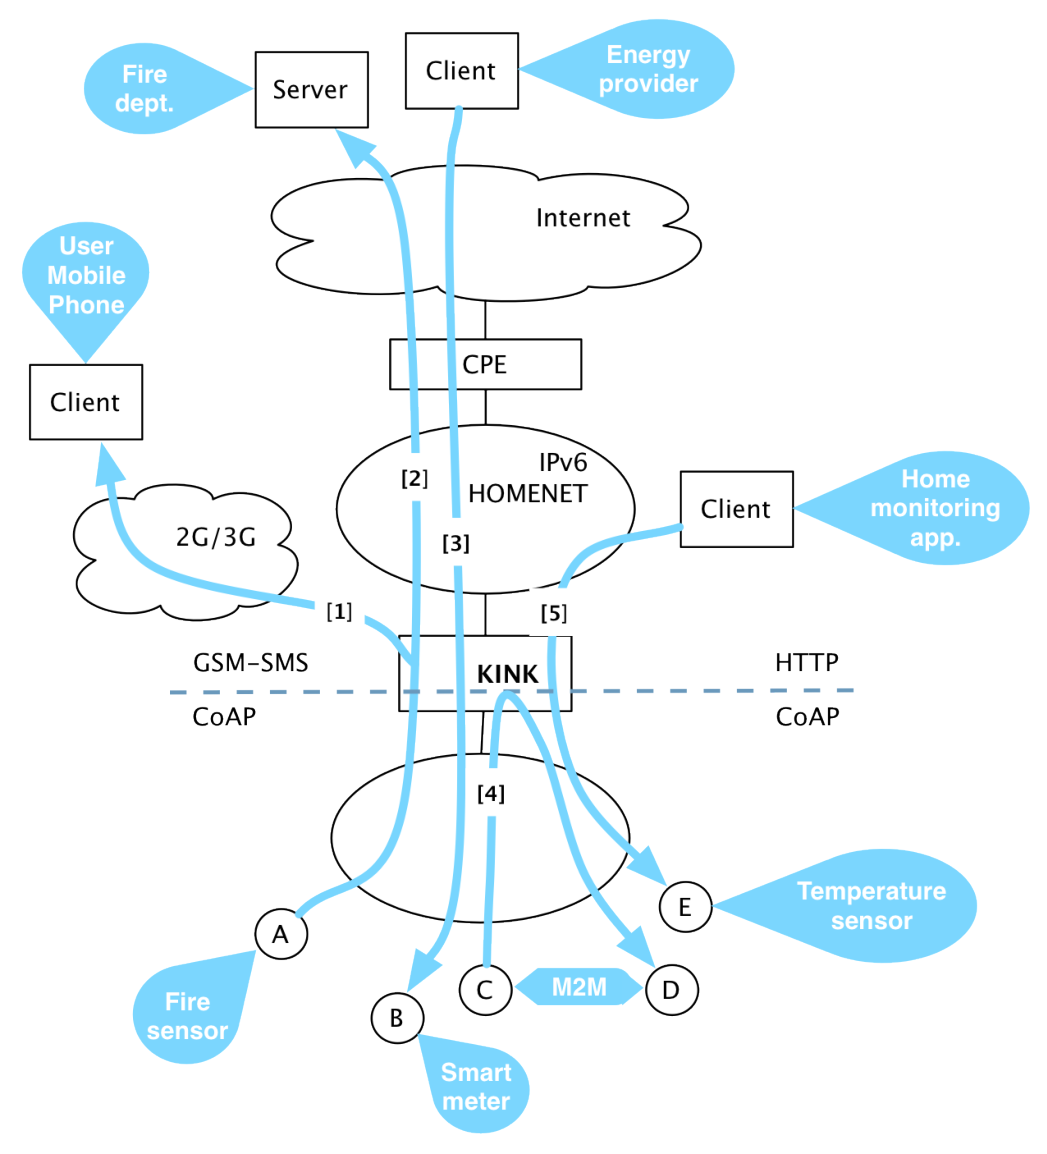
\includegraphics[width=14cm]{../share/images/kink-homenet}
            \caption{KINK architecture}
            \label{fig:arch}
    \end{figure}
\end{center}

Compared to other available solutions which are only proprietary, the advantages of applying open standards and open source to such framework should be self-evident: they promote and allow for unprecedented levels of interoperability with other systems, and extensibility of pre-existing ones. These are both key factors when such wide-usage systems are expected to constantly evolve in the direction of increasingly smart and useful solutions.


\section{CyaSSL}

\subsection{TLS items required by CoAP}
\begin{itemize}
\item \href{http://tools.ietf.org/html/rfc4347}{DTLS version 1.0} (what about 1.2 ?);
\item \href{http://tools.ietf.org/html/rfc4279}{Pre-Shared Key Ciphersuites};
\item \href{http://tools.ietf.org/html/draft-wouters-tls-oob-pubkey}{TLS out-of-band public key validation};
\end{itemize}

\subsection{Target requirements}
Target operating systems:
\begin{enumerate}
\item\label{contiki} \href{http://www.contiki-os.org}{Contiki OS} -- currently working on HEAD;
\item\label{tinyos} \href{http://www.tinyos.net}{TinyOS} -- currently working on HEAD;
\end{enumerate}

mandatory to implement \ref{contiki} which btw seems , preferably \ref{tinyos}.  

\section{Trivia}

\subsection{Zolertia Z1}
\begin{itemize}
  \item \textbf{microcontroller:} Texas Instruments MSP430F2617;
  \item \textbf{transciever:} Chipcon CC2420 2.4 GHz IEEE 802.15.4 Wireless Transceiver;
  \item \textbf{program + data mem:} 8 KB RAM;
  \item \textbf{external memory:} 92 KB Flash;
  \item \textbf{programming:} C, nesC
  \item \textbf{notes:} Contiki and TinyOS Support. 16 Mbit external flash + 2 digital on-board sensors
\end{itemize}


\subsection{Contiki OS}
Contiki is an open source, highly portable, multi-tasking operating system for memory-efficient networked embedded systems and WSN.  The core of Contiki contains several components including uIP and Sicslopan communication stacks. uIP is a small RFC-compliant TCP/IP stack that makes it possible for Contiki to communicate over the Internet, while the Sicslopan stack realizes 6LoWPAN process according to [RFC4944] and ietf-draft-6lowpan-hc-01.  Contiki is implemented in a layered structure.  The hardware platform difference is also considered by implementing drivers for different platforms.  

\subsection{TinyOS}
The currently most extensive implementation of 6LoWPAN for TinyOS (prevalent WSN operating system) is called blip developed at the University of California, Berkeley.  IPv6 neighbor discovery, default route selection and point-to-point routing are the most important features it supports.  In addition to the IPv6 functionalities, it supports ICMP, UDP and includes a prototype TCP stack.  Although it implements much functionality, it still contains several known issues.  The fragmentation of IP packets used in blip provides several problems, in particular when using multi-hop.  Buffering is a second known issue of blip.  Blip is mainly based on several message buffers and windows, which consume a large amount of memory.  This leads to several problems as messages are dropped if the buffer has no free space.  The bilp does not include standard IEEE 802.15.4 interfaces.  

\end{document}
